%% == LaTeX PACKAGE tikz-quantumgates ================================
%%    Drawing quantum circuits with TikZ
%% 
%% Matthias Wolff, BTU Cottbus-Sentenberg
%% August 20, 2018
%% DOI 
%%
%% References:
%% [1] R. Niepraschk: The showexpl package. 2016. Online, retrieved July 23, 2018. 
%%     http://mirror.ctan.org/macros/latex/contrib/showexpl/doc/showexpl.pdf
%%     http://mirror.ctan.org/macros/latex/contrib/showexpl/doc/showexpl-test.pdf
%% [2] C. Heinz, B. Moses, and J. Hoffmann. The Listings Package. 2015. Online, retrieved July 23, 2018.
%%     http://mirror.ctan.org/macros/latex/contrib/listings/listings.pdf
%%
\documentclass[a4paper]{article}
%
% Packages
\usepackage{amsmath}
\usepackage{amssymb}
\usepackage[dvipsnames]{xcolor}
\usepackage{xspace}
\usepackage{authblk}
\usepackage{url}
\usepackage{afterpage}
\usepackage{array}
\usepackage{longtable}
\usepackage{listings}
\usepackage{showexpl}
\usepackage[capitalize]{cleveref}
\usepackage{tikz}
\usepackage{tikz-quantumgates}
%
% Names
\newcommand{\Ntikz}{TikZ\xspace}
\newcommand{\Npckg}{\texttt{tikz-quantumgates}\xspace}
%
% Custom commands
\newcommand\e{\mathrm{e}}
\renewcommand\i{\mathrm{i}}
\newcommand\atann{\mathop{\operatorname{arctan2}}}
\newcommand{\TT}[1]{\protect\scalebox{0.75}[1.04]{\texttt{#1}}}
\newcommand{\CORR}[1]{{\color{red!90!RoyalBlue}#1}}
\newcommand{\workOn}{\color{Salmon!80!black}}
\newcommand{\workOff}{\color{black}}
\newcommand{\TODO}[1]{%
  \fboxsep=1pt\fboxrule=1pt\fcolorbox{yellow}{white}{[\textbf{TODO:~}#1]}%
}
\newcommand{\CHECK}[1]{%
  \fboxsep=1pt\fboxrule=1pt\fcolorbox{yellow}{white}{#1}%
}
\newcommand\docCmd[2]{%
  \pagebreak[1]\bigskip\noindent%
  \fboxsep=3pt
  \fcolorbox{black!15}{black!15}{\parbox{\linewidth}{%
    \texttt{\textbackslash #1}}%
  }%
  \addcontentsline{toc}{subsubsection}{\texttt{\textbackslash #1}}%
  
  \bigskip\noindent #2
}
\newcommand\docPar[2]{{%
  \renewcommand\arraystretch{1.15}
  \begin{tabular}{p{40pt}p{370pt}}
    \texttt{#1} & #2
  \end{tabular}%
}}
%
% Settings
% - Page layout
\renewcommand{\floatpagefraction}{.8}
\textheight242mm
\textwidth150mm
\marginparwidth28mm
\topmargin-15mm
\oddsidemargin0mm
\evensidemargin0mm
% - Listings
\renewcommand{\lstlistingname}{Example}
\lstdefinestyle{lstsMatlab}{%
  basicstyle=\footnotesize\ttfamily,%
    backgroundcolor=\color{black!5},%
    basewidth=0.47em, fontadjust, columns=fixed,%
    numbers=left, numberstyle=\sffamily\tiny, numbersep=2pt,%
  language=Matlab,
    commentstyle=\color{OliveGreen!60!black},%\itshape,%
}
\lstdefinestyle{lstsLatex}{%
  basicstyle=\footnotesize\ttfamily,%
    backgroundcolor=\color{black!5},%
    basewidth=0.47em, fontadjust, columns=fixed,%
    numbers=left, numberstyle=\sffamily\tiny, numbersep=2pt,%
  language=[LaTeX]TeX,%
    mathescape=false,escapechar=�,%
    commentstyle=\color{OliveGreen!60!black},%\itshape,%
    keywordstyle=\color{blue},%
    texcsstyle=*\color{RoyalPurple}\bfseries,%
    moretexcs={%
      color,%
      node,%
      draw,%
      ifthenelse,%
      coordinate,%
      pgfmathsetmacro,%
      qScalePaper,%
      tikzset,%
      isin,%
      qwire,%
      qzero,%
      qgateControl,%
      qgateU,%
      qgateUu,%
      qgateUuu,%
      qgateID,%
      qgateX,%
      qgateY,%
      qgateZ,%
      qgateH,%
      qgateS,%
      qgateSi,%
      qgateT,%
      qgateTi,%
      qgateUa,%
      qgateUb,%
      qgateUc,%
      qgateCNX,%
      qgateCNC,%
      qgateCNR,%
      qgateOID,%
      qmeasM,%
      qmeasR,%
      qmeasMB,%
      qmeasB,%
      qmeasBh,%
      qgateOX,%
      qgateOY,%
      qgateOZ,%
      qgateOH,%
      qgateOS,%
      qgateOSi,%
      qgateOT,%
      qgateOTi,%
      qgateOUa,%
      qgateOUb,%
      qgateOUc,%
      qgateOCNOT,%
      qgateOCCNOT,%
    },%
    deletetexcs={%
    },%
    stringstyle=\color{Orange},
    showstringspaces=false,
    morestring=[s]{[}{]},
}
\lstdefinestyle{lstsFrontPage}{
  style=lstsLatex,
  basicstyle=\scriptsize\ttfamily,
  basewidth=0.42em,
  pos=t,
  rframe=,
  varwidth=true, justification=\centering
}
\lstdefinestyle{lstsNormalLines}{
  style=lstsLatex,
  pos=t,
  rframe=,
  varwidth=true, justification=\centering
}
\lstdefinestyle{lstsLongLines}{
  style=lstsLatex,
  overhang={55pt},
  pos=t,
  rframe=,
  varwidth=true, justification=\centering
}
\lstdefinestyle{lstsDocExamples}{
  style=lstsLatex,
  overhang={7pt},
  pos=l,
  rframe=,
  varwidth=true
}
% - Other
\setcounter{secnumdepth}{2}

%%%%%%%%%%%%%%%%%%%%%%%%%%%%%%%%%%%%%%%%%%%%%%%%%%%%%%%%%%%%%%%%%%%%%%%%%%%%%%%

\begin{document}
%
\author{Matthias Wolff$^{\text{\sf\,[0000--0002--3895--7313]}}$}
\affil{BTU Cottbus-Senftenberg}
\title{The \Npckg Package:\\
Drawing quantum circuits with \Ntikz}
\maketitle

\bigskip\noindent
See \TT{https://github.com/matthias-wolff/tikz-quantumgates/blob/master/tikz-quantumgates.pdf}
for the latest version of this document.
\begin{center}
  \bigskip\bigskip
  \begin{minipage}{0.9\linewidth}
    \textbf{Abstract}

    \bigskip
    This package provides macros for drawing quantum gates and circuits with
    \Ntikz \cite{Tan15}.

  \end{minipage}
  \vfill
  \begin{tabular}{@{\extracolsep{-10pt}}cc}
    \parbox[t]{220pt}{
      \LTXinputExample[style=lstsFrontPage]{example_frontpage1}
    }
  & \parbox[t]{220pt}{
      %\vspace*{-8pt}
      \LTXinputExample[style=lstsFrontPage,overhang={20pt}]{example_frontpage2}
    }
  \end{tabular}
  \vfill
\end{center}
\clearpage

\tableofcontents
\clearpage

%%%%%%%%%%%%%%%%%%%%%%%%%%%%%%%%%%%%%%%%%%%%%%%%%%%%%%%%%%%%%%%%%%%%%%%%%%%%%%%

\section{Overview}
\subsection{List of Circuit Symbols}
\begin{longtable}{m{40pt}m{60pt}p{295pt}}
  \hline Standard & Option \texttt{ibmqx} & Command \\\hline 
\endfirsthead
  \multicolumn{3}{l}{{Continued from previous page}} \\\hline 
  Standard & Option \texttt{ibmqx} & Command \\\hline 
  \multicolumn{3}{r}{~} \\[-9pt]
\endhead
  \hline \multicolumn{3}{r}{{Continued on next page}} \\
\endfoot
  \hline 
\endlastfoot
  \centering\tikz{\qwire{0}{0}} & 
  \centering\tikz{\qwire[ibmqx]{0}{0}} & 
  \texttt{\textbackslash qwire[option]\{x\}\{y\}}
\\ 
  \centering\tikz{\qzero{0}{0}} & 
  \centering\tikz{\qzero[ibmqx]{0}{0}} & 
  \texttt{\textbackslash qzero[option]\{x\}\{y\}}
\\ 
  \centering\tikz{\qgateID{0}{0}} &
  \centering\tikz{\qgateID[ibmqx]{0}{0}} & 
  \texttt{\textbackslash qgateID[option]\{x\}\{y\}}
\\ 
  \centering\tikz{\qgateX{0}{0}} &
  \centering\tikz{\qgateX[ibmqx]{0}{0}} & 
  \texttt{\textbackslash qgateX[option]\{x\}\{y\}}
\\ 
  \centering\tikz{\qgateY{0}{0}} &
  \centering\tikz{\qgateY[ibmqx]{0}{0}} & 
  \texttt{\textbackslash qgateY[option]\{x\}\{y\}}
\\ 
  \centering\tikz{\qgateZ{0}{0}} &
  \centering\tikz{\qgateZ[ibmqx]{0}{0}} & 
  \texttt{\textbackslash qgateZ[option]\{x\}\{y\}}
\\ 
  \centering\tikz{\qgateH{0}{0}} &
  \centering\tikz{\qgateH[ibmqx]{0}{0}} & 
  \texttt{\textbackslash qgateH[option]\{x\}\{y\}}
\\ 
  \centering\tikz{\qgateS{0}{0}} &
  \centering\tikz{\qgateS[ibmqx]{0}{0}} & 
  \texttt{\textbackslash qgateS[option]\{x\}\{y\}}
\\ 
  \centering\tikz{\qgateSi{0}{0}} &
  \centering\tikz{\qgateSi[ibmqx]{0}{0}} & 
  \texttt{\textbackslash qgateSi[option]\{x\}\{y\}}
\\ 
  \centering\tikz{\qgateT{0}{0}} &
  \centering\tikz{\qgateT[ibmqx]{0}{0}} & 
  \texttt{\textbackslash qgateT[option]\{x\}\{y\}}
\\
  \centering\tikz{\qgateTi{0}{0}} &
  \centering\tikz{\qgateTi[ibmqx]{0}{0}} & 
  \texttt{\textbackslash qgateTi[option]\{x\}\{y\}}
\\ 
  \centering\tikz{\qgateUa{0}{0}} &
  \centering\tikz{\qgateUa[ibmqx]{0}{0}} & 
  \texttt{\textbackslash qgateUa[option]\{x\}\{y\}}
\\ 
  \centering\tikz{\qgateUb{0}{0}} &
  \centering\tikz{\qgateUb[ibmqx]{0}{0}} & 
  \texttt{\textbackslash qgateUb[option]\{x\}\{y\}}
\\ 
  \centering\tikz{\qgateUc{0}{0}} &
  \centering\tikz{\qgateUc[ibmqx]{0}{0}} & 
  \texttt{\textbackslash qgateUc[option]\{x\}\{y\}}
\\ 
  \centering\tikz{\qgateUa*{0}{0}{$\lambda$}} &
  \centering\tikz{\qgateUa*[ibmqx]{0}{0}{$\lambda$}} & 
  \texttt{\textbackslash qgateUa*[option]\{x\}\{y\}\{sublabel\}}
\\ 
  \centering\tikz{\qgateUb*{0}{0}{$\lambda,\phi$}} &
  \centering\tikz{\qgateUb*[ibmqx]{0}{0}{$\lambda,\phi$}} & 
  \texttt{\textbackslash qgateUb*[option]\{x\}\{y\}\{sublabel\}}
\\ 
  \centering\tikz{\qgateUc*{0}{0}{$\theta,\lambda,\phi$}} &
  \centering\tikz{\qgateUc*[ibmqx]{0}{0}{$\theta,\lambda,\phi$}} & 
  \texttt{\textbackslash qgateUc*[option]\{x\}\{y\}\{sublabel\}}
\\ 
  \centering\tikz{\qgateCNX{b}{0}{0}} &
  \centering\tikz{\qgateCNX[ibmqx]{b}{0}{0}} & 
  \texttt{\textbackslash qgateCNX[option]\{cwires\}\{x\}\{y\}}
\\ 
  \centering\tikz{\qgateCNR{0}{0}} &
  \centering\tikz{\qgateCNR[ibmqx]{0}{0}} & 
  \texttt{\textbackslash qgateCNR[option]\{x\}\{y\}}
\\ 
  \centering\tikz{\qgateCNC{t}{0}{0}} &
  \centering\tikz{\qgateCNC[ibmqx]{t}{0}{0}} & 
  \texttt{\textbackslash qgateCNC[option]\{cwires\}\{x\}\{y\}}
\\ 
  \centering\tikz{\qgateSWt{0}{0}} &
  \centering$\begin{pmatrix}\tikz{\qgateSWt[ibmqx]{0}{0}}\end{pmatrix}$ & 
  \texttt{\textbackslash qgateSWt[option]\{x\}\{y\}}
  {\footnotesize (not an ``official'' IBM QX symbol)}
\\ 
  \centering\tikz{\qgateSWR{0}{0}} &
  \centering$\begin{pmatrix}\tikz{\qgateSWR[ibmqx]{0}{0}}\end{pmatrix}$ & 
  \texttt{\textbackslash qgateSWR[option]\{x\}\{y\}}
  {\footnotesize (not an ``official'' IBM QX symbol)}
\\ 
  \centering\tikz{\qgateSWb{0}{0}} &
  \centering$\begin{pmatrix}\tikz{\qgateSWb[ibmqx]{0}{0}}\end{pmatrix}$ & 
  \texttt{\textbackslash qgateSWb[option]\{x\}\{y\}}
  {\footnotesize (not an ``official'' IBM QX symbol)}
\\ 
  \centering\tikz{\qmeasM{0}{0}} &
  \centering\tikz{\qmeasM[ibmqx]{0}{0}} & 
  \texttt{\textbackslash qmeasM[option]\{x\}\{y\}}
\\ 
  \centering\tikz{\qmeasM*{0}{0}{X}{b}} &
  \centering\tikz{\qmeasM*[ibmqx]{0}{0}{X}{b}} & 
  \texttt{\textbackslash qmeasM*[option]\{x\}\{y\}\{axis\}\{wires\}}
\\ 
  \centering\tikz{\qmeasR{0}{0}} &
  \centering\tikz{\qmeasR[ibmqx]{0}{0}} & 
  \texttt{\textbackslash qmeasR[option]\{x\}\{y\}}
\\ 
  \centering\tikz{\qmeasMB{0}{0}{0}} &
  \centering\tikz{\qmeasMB[ibmqx]{0}{0}{0}} & 
  \texttt{\textbackslash qmeasMB[option]\{b\}\{x\}\{y\}}
\\ 
  \centering\tikz{\qmeasB{0}{0}} &
  \centering\tikz{\qmeasB[ibmqx]{0}{0}} & 
  \texttt{\textbackslash qmeasB[option]\{x\}\{y\}}
\\ 
  \centering\tikz{\qmeasBh{0}{0}{0}} &
  \centering\tikz{\qmeasBh[ibmqx]{0}{0}{0}} & 
  \texttt{\textbackslash qmeasBh[option]\{b\}\{x\}\{y\}}
\\ 
  \centering\tikz{\qgateU{0}{0}{U}} &
  \centering$\begin{pmatrix}\tikz{\qgateU[ibmqx]{0}{0}{U}}\end{pmatrix}$ & 
  \texttt{\textbackslash qgateU[option]\{x\}\{y\}\{label\}}
  {\footnotesize (not an ``official'' IBM QX symbol)}
\\ 
  \centering\tikz{\qgateUu{0}{0}{U}} &
  \centering$\begin{pmatrix}\tikz{\qgateUu[ibmqx]{0}{0}{U}}\end{pmatrix}$ & 
  \texttt{\textbackslash qgateUu[option]\{x\}\{y\}\{label\}}
  {\footnotesize (not an ``official'' IBM QX symbol)}
\\ 
  \centering\tikz{\qgateUuu{0}{0}{U}} &
  \centering$\begin{pmatrix}\tikz{\qgateUuu[ibmqx]{0}{0}{U}}\end{pmatrix}$ & 
  \texttt{\textbackslash qgateUuu[option]\{x\}\{y\}\{label\}}
  {\footnotesize (not an ``official'' IBM QX symbol)}
\end{longtable}

Any gate can be equipped with control wires, e.g.
\begin{longtable}{m{40pt}m{60pt}p{295pt}}
  \centering\tikz{\qgateUc{0}{0};\qgateControl{t}{0}{0};} &
  \centering\tikz{\qgateUc[ibmqx]{0}{0};\qgateControl[ibmqxA]{t}{0}{0};} & 
  \texttt{\textbackslash qgateUc[option]\{x\}\{y\}\textbackslash qgateControl[option]\{cwires\}\{x\}\{y\}}
\end{longtable}

\subsection{Installation}
Download \texttt{\Npckg.sty} from \cite{Wol18} file into your project folder
and include the package with \texttt{\textbackslash
usepackage\{\Npckg\!\!\!\}}.

%%%%%%%%%%%%%%%%%%%%%%%%%%%%%%%%%%%%%%%%%%%%%%%%%%%%%%%%%%%%%%%%%%%%%%%%%%%%%%%

\section{Documentation of Commands}
\subsection{Wire and State Preparation Symbols}

%% == \qwire ==================================================================
\docCmd{qwire[option]\{x\}\{y\}}{%
  Draws a wire.
}
\subsubsection*{Parameters}
\docPar{option}{%
  Omit for standard circuit styling or \texttt{ibmqx} for IBM Q Experience
  circuit styling.
}
\docPar{x, y}{%
  Position of symbol in schematic. The actual \Ntikz coordinates are
  $(\texttt{\textbackslash qgateSx*x},\texttt{y})$.
}

\subsubsection*{Examples}
\begin{LTXexample}[style=lstsDocExamples]
\begin{tikzpicture}
  \qScalePaper
  \qwire{0}{0}
\end{tikzpicture}
\end{LTXexample}
\begin{LTXexample}[style=lstsDocExamples]
\begin{tikzpicture}
  \qScalePaper
  \qwire[ibmqx]{0}{0}
\end{tikzpicture}
\end{LTXexample}

%% == \qzero ==================================================================
\docCmd{qzero[option]\{x\}\{y\}}{%
  Draws the zero-state preparator.
}
\subsubsection*{Parameters}
\docPar{option}{%
  Omit for standard circuit styling or \texttt{ibmqx} for IBM Q Experience
  circuit styling.
}
\docPar{x, y}{%
  Position of symbol in schematic. The actual \Ntikz coordinates are
  $(\texttt{\textbackslash qgateSx*x},\texttt{y})$.
}

\subsubsection*{Examples}
\begin{LTXexample}[style=lstsDocExamples]
\begin{tikzpicture}
  \qScalePaper
  \qzero{0}{0}
\end{tikzpicture}
\end{LTXexample}
\begin{LTXexample}[style=lstsDocExamples]
\begin{tikzpicture}
  \qScalePaper
  \qzero[ibmqx]{0}{0}
\end{tikzpicture}
\end{LTXexample}

%%%%%%%%%%%%%%%%%%%%%%%%%%%%%%%%%%%%%%%%%%%%%%%%%%%%%%%%%%%%%%%%%%%%%%%%%%%%%%%

\subsection{Single-Qubit Gate Symbols}

%% == \qgateU =================================================================
\docCmd{qgateU[option]\{x\}\{y\}\{label\}}{%
  Draws a general single-qubit quantum gate.
}

\subsubsection*{Parameters}
\docPar{option}{%
  Omit for standard circuit styling or \texttt{ibmqxA},\ldots,\texttt{ibmqxH}
  for IBM Q Experience circuit styling. The last letter of \texttt{ibmqx*}
  defines the color of the gate symbol:

  \vspace*{6pt}
  \tikz{\fill[ibmqxA] (-0.2,-0.2) rectangle (0.2,0.2); \node[white] at (0,0) {\texttt{A}};}
  \tikz{\fill[ibmqxB] (-0.2,-0.2) rectangle (0.2,0.2); \node[white] at (0,0) {\texttt{B}};}
  \tikz{\fill[ibmqxC] (-0.2,-0.2) rectangle (0.2,0.2); \node[white] at (0,0) {\texttt{C}};}
  \tikz{\fill[ibmqxD] (-0.2,-0.2) rectangle (0.2,0.2); \node[white] at (0,0) {\texttt{D}};}
  \tikz{\fill[ibmqxE] (-0.2,-0.2) rectangle (0.2,0.2); \node[white] at (0,0) {\texttt{E}};}
  \tikz{\fill[ibmqxF] (-0.2,-0.2) rectangle (0.2,0.2); \node[white] at (0,0) {\texttt{F}};}
  \tikz{\fill[ibmqxG] (-0.2,-0.2) rectangle (0.2,0.2); \node[white] at (0,0) {\texttt{G}};}
  \tikz{\fill[ibmqxH] (-0.2,-0.2) rectangle (0.2,0.2); \node[black] at (0,0) {\texttt{H}};}

  If \texttt{ibmqx} is passed, \texttt{ibmqxG} will be used.
}
\docPar{x, y}{%
  Position of symbol in schematic. The actual \Ntikz coordinates are
  $(\texttt{\textbackslash qgateSx*x},\texttt{y})$.
}
\docPar{label}{%
  Gate label.
}

\subsubsection*{Examples}
\begin{LTXexample}[style=lstsDocExamples]
\begin{tikzpicture}
  \qScalePaper
  \qgateU{0}{0}{U1}
\end{tikzpicture}
\end{LTXexample}
\begin{LTXexample}[style=lstsDocExamples]
\begin{tikzpicture}
  \qScalePaper
  \qgateU[ibmqxA]{0}{0}{U1}
\end{tikzpicture}
\end{LTXexample}

%% == \qgateID =================================================================
\docCmd{qgateID[option]\{x\}\{y\}}{%
  Draws the identity gate.
}

\subsubsection*{Parameters}
\docPar{option}{%
  Omit for standard circuit styling or \texttt{ibmqx} for IBM Q Experience
  circuit styling.
}
\docPar{x, y}{%
  Position of symbol in schematic. The actual \Ntikz coordinates are
  $(\texttt{\textbackslash qgateSx*x},\texttt{y})$.
}

\subsubsection*{Examples}
\begin{LTXexample}[style=lstsDocExamples]
\begin{tikzpicture}
  \qScalePaper
  \qgateID{0}{0}
\end{tikzpicture}
\end{LTXexample}
\begin{LTXexample}[style=lstsDocExamples]
\begin{tikzpicture}
  \qScalePaper
  \qgateID[ibmqx]{0}{0}
\end{tikzpicture}
\end{LTXexample}

\subsubsection*{Gate Operator}
\begin{LTXexample}[style=lstsDocExamples]
  $\displaystyle I\doteq\qgateOID $
\end{LTXexample}

%% == \qgateX =================================================================
\docCmd{qgateX[option]\{x\}\{y\}}{%
  Pauli-X gate.
}

\subsubsection*{Parameters}
\docPar{option}{%
  Omit for standard circuit styling or \texttt{ibmqx} for IBM Q Experience
  circuit styling.
}
\docPar{x, y}{%
  Position of symbol in schematic. The actual \Ntikz coordinates are
  $(\texttt{\textbackslash qgateSx*x},\texttt{y})$.
}

\subsubsection*{Examples}
\begin{LTXexample}[style=lstsDocExamples]
\begin{tikzpicture}
  \qScalePaper
  \qgateX{0}{0}
\end{tikzpicture}
\end{LTXexample}
\begin{LTXexample}[style=lstsDocExamples]
\begin{tikzpicture}
  \qScalePaper
  \qgateX[ibmqx]{0}{0}
\end{tikzpicture}
\end{LTXexample}

\subsubsection*{Gate Operator}
\begin{LTXexample}[style=lstsDocExamples]
  $\displaystyle X\doteq\qgateOX $
\end{LTXexample}

%% == \qgateY =================================================================
\docCmd{qgateY[option]\{x\}\{y\}}{%
  Pauli-Y gate.
}

\subsubsection*{Parameters}
\docPar{option}{%
  Omit for standard circuit styling or \texttt{ibmqx} for IBM Q Experience
  circuit styling.
}
\docPar{x, y}{%
  Position of symbol in schematic. The actual \Ntikz coordinates are
  $(\texttt{\textbackslash qgateSx*x},\texttt{y})$.
}

\subsubsection*{Examples}
\begin{LTXexample}[style=lstsDocExamples]
\begin{tikzpicture}
  \qScalePaper
  \qgateY{0}{0}
\end{tikzpicture}
\end{LTXexample}
\begin{LTXexample}[style=lstsDocExamples]
\begin{tikzpicture}
  \qScalePaper
  \qgateY[ibmqx]{0}{0}
\end{tikzpicture}
\end{LTXexample}

\subsubsection*{Gate Operator}
\begin{LTXexample}[style=lstsDocExamples]
  $\displaystyle Y\doteq\qgateOY $
\end{LTXexample}

%% == \qgateZ =================================================================
\docCmd{qgateZ[option]\{x\}\{y\}}{%
  Pauli-Z gate.
}

\subsubsection*{Parameters}
\docPar{option}{%
  Omit for standard circuit styling or \texttt{ibmqx} for IBM Q Experience
  circuit styling.
}
\docPar{x, y}{%
  Position of symbol in schematic. The actual \Ntikz coordinates are
  $(\texttt{\textbackslash qgateSx*x},\texttt{y})$.
}

\subsubsection*{Examples}
\begin{LTXexample}[style=lstsDocExamples]
\begin{tikzpicture}
  \qScalePaper
  \qgateZ{0}{0}
\end{tikzpicture}
\end{LTXexample}
\begin{LTXexample}[style=lstsDocExamples]
\begin{tikzpicture}
  \qScalePaper
  \qgateZ[ibmqx]{0}{0}
\end{tikzpicture}
\end{LTXexample}

\subsubsection*{Gate Operator}
\begin{LTXexample}[style=lstsDocExamples]
  $\displaystyle Z\doteq\qgateOZ $
\end{LTXexample}

%% == \qgateH =================================================================
\docCmd{qgateH[option]\{x\}\{y\}}{%
  Hadamard gate.
}

\subsubsection*{Parameters}
\docPar{option}{%
  Omit for standard circuit styling or \texttt{ibmqx} for IBM Q Experience
  circuit styling.
}
\docPar{x, y}{%
  Position of symbol in schematic. The actual \Ntikz coordinates are
  $(\texttt{\textbackslash qgateSx*x},\texttt{y})$.
}

\subsubsection*{Examples}
\begin{LTXexample}[style=lstsDocExamples]
\begin{tikzpicture}
  \qScalePaper
  \qgateH{0}{0}
\end{tikzpicture}
\end{LTXexample}
\begin{LTXexample}[style=lstsDocExamples]
\begin{tikzpicture}
  \qScalePaper
  \qgateH[ibmqx]{0}{0}
\end{tikzpicture}
\end{LTXexample}

\subsubsection*{Gate Operator}
\begin{LTXexample}[style=lstsDocExamples]
$\displaystyle H\doteq\qgateOH $
\end{LTXexample}

%% == \qgateS =================================================================
\docCmd{qgateS[option]\{x\}\{y\}}{%
  S phase gate.
}

\subsubsection*{Parameters}
\docPar{option}{%
  Omit for standard circuit styling or \texttt{ibmqx} for IBM Q Experience
  circuit styling.
}
\docPar{x, y}{%
  Position of symbol in schematic. The actual \Ntikz coordinates are
  $(\texttt{\textbackslash qgateSx*x},\texttt{y})$.
}

\subsubsection*{Examples}
\begin{LTXexample}[style=lstsDocExamples]
\begin{tikzpicture}
  \qScalePaper
  \qgateS{0}{0}
\end{tikzpicture}
\end{LTXexample}
\begin{LTXexample}[style=lstsDocExamples]
\begin{tikzpicture}
  \qScalePaper
  \qgateS[ibmqx]{0}{0}
\end{tikzpicture}
\end{LTXexample}

\subsubsection*{Gate Operator}
\begin{LTXexample}[style=lstsDocExamples]
$\displaystyle S=\sqrt{Z}\doteq\qgateOS $
\end{LTXexample}

%% == \qgateSi ================================================================
\docCmd{qgateSi[option]\{x\}\{y\}}{%
  Inverse S phase gate.
}

\subsubsection*{Parameters}
\docPar{option}{%
  Omit for standard circuit styling or \texttt{ibmqx} for IBM Q Experience
  circuit styling.
}
\docPar{x, y}{%
  Position of symbol in schematic. The actual \Ntikz coordinates are
  $(\texttt{\textbackslash qgateSx*x},\texttt{y})$.
}

\subsubsection*{Examples}
\begin{LTXexample}[style=lstsDocExamples]
\begin{tikzpicture}
  \qScalePaper
  \qgateSi{0}{0}
\end{tikzpicture}
\end{LTXexample}
\begin{LTXexample}[style=lstsDocExamples]
\begin{tikzpicture}
  \qScalePaper
  \qgateSi[ibmqx]{0}{0}
\end{tikzpicture}
\end{LTXexample}

\subsubsection*{Gate Operator}
\begin{LTXexample}[style=lstsDocExamples]
$\displaystyle S^\dagger\doteq\qgateOSi $
\end{LTXexample}

%% == \qgateT =================================================================
\docCmd{qgateT[option]\{x\}\{y\}}{%
  T phase gate.
}

\subsubsection*{Parameters}
\docPar{option}{%
  Omit for standard circuit styling or \texttt{ibmqx} for IBM Q Experience
  circuit styling.
}
\docPar{x, y}{%
  Position of symbol in schematic. The actual \Ntikz coordinates are
  $(\texttt{\textbackslash qgateSx*x},\texttt{y})$.
}

\subsubsection*{Examples}
\begin{LTXexample}[style=lstsDocExamples]
\begin{tikzpicture}
  \qScalePaper
  \qgateT{0}{0}
\end{tikzpicture}
\end{LTXexample}
\begin{LTXexample}[style=lstsDocExamples]
\begin{tikzpicture}
  \qScalePaper
  \qgateT[ibmqx]{0}{0}
\end{tikzpicture}
\end{LTXexample}

\subsubsection*{Gate Operator}
\begin{LTXexample}[style=lstsDocExamples]
$\displaystyle T=\sqrt{S}\doteq\qgateOT $
\end{LTXexample}

%% == \qgateTi ================================================================
\docCmd{qgateTi[option]\{x\}\{y\}}{%
  Inverse T phase gate.
}

\subsubsection*{Parameters}
\docPar{option}{%
  Omit for standard circuit styling or \texttt{ibmqx} for IBM Q Experience
  circuit styling.
}
\docPar{x, y}{%
  Position of symbol in schematic. The actual \Ntikz coordinates are
  $(\texttt{\textbackslash qgateSx*x},\texttt{y})$.
}

\subsubsection*{Examples}
\begin{LTXexample}[style=lstsDocExamples]
\begin{tikzpicture}
  \qScalePaper
  \qgateTi{0}{0}
\end{tikzpicture}
\end{LTXexample}
\begin{LTXexample}[style=lstsDocExamples]
\begin{tikzpicture}
  \qScalePaper
  \qgateTi[ibmqx]{0}{0}
\end{tikzpicture}
\end{LTXexample}

\subsubsection*{Gate Operator}
\begin{LTXexample}[style=lstsDocExamples]
$\displaystyle T^\dagger\doteq\qgateOTi $
\end{LTXexample}

%%%%%%%%%%%%%%%%%%%%%%%%%%%%%%%%%%%%%%%%%%%%%%%%%%%%%%%%%%%%%%%%%%%%%%%%%%%%%%%

\subsection{Single-Qubit Physical Gate of IBM Q Experience}

%% == \qgateUa ================================================================
\docCmd{qgateUa[option]\{x\}\{y\}\\\textbackslash qgateUa*[option]\{x\}\{y\}\{sublabel\}}{%
  U1 gate of IBM Q Experience.
}

\subsubsection*{Parameters}
\docPar{option}{%
  Omit for standard circuit styling or \texttt{ibmqx} for IBM Q Experience
  circuit styling.
}
\docPar{x, y}{%
  Position of symbol in schematic. The actual \Ntikz coordinates are
  $(\texttt{\textbackslash qgateSx*x},\texttt{y})$.
}
\docPar{sublabel}{%
  Sub-label, e.\,g. for gate parameters (starred version only) 
}

\subsubsection*{Examples}
\begin{LTXexample}[style=lstsDocExamples]
\begin{tikzpicture}
  \qScalePaper
  \qgateUa{0}{0}
\end{tikzpicture}
\end{LTXexample}
\begin{LTXexample}[style=lstsDocExamples]
\begin{tikzpicture}
  \qScalePaper
  \qgateUa[ibmqx]{0}{0}
\end{tikzpicture}
\end{LTXexample}
\begin{LTXexample}[style=lstsDocExamples]
\begin{tikzpicture}
  \qScalePaper
  \qgateUa*{0}{0}{$\lambda$}
\end{tikzpicture}
\end{LTXexample}
\begin{LTXexample}[style=lstsDocExamples]
\begin{tikzpicture}
  \qScalePaper
  \qgateUa*[ibmqx]{0}{0}{$\lambda$}
\end{tikzpicture}
\end{LTXexample}

\subsubsection*{Gate Operator}
\begin{LTXexample}[style=lstsDocExamples]
$\displaystyle U1_{\lambda}\doteq\qgateOUa $
\end{LTXexample}

%% == \qgateUb ================================================================
\docCmd{qgateUb[option]\{x\}\{y\}\\\textbackslash qgateUb*[option]\{x\}\{y\}\{sublabel\}}{%
  U2 gate of IBM Q Experience.
}

\subsubsection*{Parameters}
\docPar{option}{%
  Omit for standard circuit styling or \texttt{ibmqx} for IBM Q Experience
  circuit styling.
}
\docPar{x, y}{%
  Position of symbol in schematic. The actual \Ntikz coordinates are
  $(\texttt{\textbackslash qgateSx*x},\texttt{y})$.
}
\docPar{sublabel}{%
  Sub-label, e.\,g. for gate parameters (starred version only) 
}

\subsubsection*{Examples}
\begin{LTXexample}[style=lstsDocExamples]
\begin{tikzpicture}
  \qScalePaper
  \qgateUb{0}{0}
\end{tikzpicture}
\end{LTXexample}
\begin{LTXexample}[style=lstsDocExamples]
\begin{tikzpicture}
  \qScalePaper
  \qgateUb[ibmqx]{0}{0}
\end{tikzpicture}
\end{LTXexample}
\begin{LTXexample}[style=lstsDocExamples]
\begin{tikzpicture}
  \qScalePaper
  \qgateUb*{0}{0}{$\lambda,\phi$}
\end{tikzpicture}
\end{LTXexample}
\begin{LTXexample}[style=lstsDocExamples]
\begin{tikzpicture}
  \qScalePaper
  \qgateUb*[ibmqx]{0}{0}{$\lambda,\phi$}
\end{tikzpicture}
\end{LTXexample}

\subsubsection*{Gate Operator}
\begin{LTXexample}[style=lstsDocExamples]
$\displaystyle U2_{\lambda,\phi}\doteq\qgateOUb $
\end{LTXexample}

%% == \qgateUc ================================================================
\docCmd{qgateUc[option]\{x\}\{y\}\\\textbackslash qgateUc*[option]\{x\}\{y\}\{sublabel\}}{%
  U3 gate of IBM Q Experience.
}

\subsubsection*{Parameters}
\docPar{option}{%
  Omit for standard circuit styling or \texttt{ibmqx} for IBM Q Experience
  circuit styling.
}
\docPar{x, y}{%
  Position of symbol in schematic. The actual \Ntikz coordinates are
  $(\texttt{\textbackslash qgateSx*x},\texttt{y})$.
}
\docPar{sublabel}{%
  Sub-label, e.\,g. for gate parameters (starred version only) 
}

\subsubsection*{Examples}
\begin{LTXexample}[style=lstsDocExamples]
\begin{tikzpicture}
  \qScalePaper
  \qgateUc{0}{0}
\end{tikzpicture}
\end{LTXexample}
\begin{LTXexample}[style=lstsDocExamples]
\begin{tikzpicture}
  \qScalePaper
  \qgateUc[ibmqx]{0}{0}
\end{tikzpicture}
\end{LTXexample}
\begin{LTXexample}[style=lstsDocExamples]
\begin{tikzpicture}
  \qScalePaper
  \qgateUc*{0}{0}{$\theta,\lambda,\phi$}
\end{tikzpicture}
\end{LTXexample}
\begin{LTXexample}[style=lstsDocExamples]
\begin{tikzpicture}
  \qScalePaper
  \qgateUc*[ibmqx]{0}{0}{$\theta,\lambda,\phi$}
\end{tikzpicture}
\end{LTXexample}

\subsubsection*{Gate Operator}
\begin{LTXexample}[style=lstsDocExamples]
$\displaystyle U3_{\lambda,\phi,\theta}\doteq\qgateOUc $
\end{LTXexample}

%%%%%%%%%%%%%%%%%%%%%%%%%%%%%%%%%%%%%%%%%%%%%%%%%%%%%%%%%%%%%%%%%%%%%%%%%%%%%%%

\subsection{Multiple-Qubit Gate Symbols}

%% == \qgateUu ================================================================
\docCmd{qgateUu[option]\{x\}\{y\}\{label\}}{%
  General three-qubit gate.
}

\subsubsection*{Parameters}
\docPar{option}{%
  Omit for standard circuit styling or \texttt{ibmqxA},\ldots,\texttt{ibmqxH}
  for IBM Q Experience circuit styling. The last letter of \texttt{ibmqx*}
  defines the color of the gate symbol:

  \vspace*{6pt}
  \tikz{\fill[ibmqxA] (-0.2,-0.2) rectangle (0.2,0.2); \node[white] at (0,0) {\texttt{A}};}
  \tikz{\fill[ibmqxB] (-0.2,-0.2) rectangle (0.2,0.2); \node[white] at (0,0) {\texttt{B}};}
  \tikz{\fill[ibmqxC] (-0.2,-0.2) rectangle (0.2,0.2); \node[white] at (0,0) {\texttt{C}};}
  \tikz{\fill[ibmqxD] (-0.2,-0.2) rectangle (0.2,0.2); \node[white] at (0,0) {\texttt{D}};}
  \tikz{\fill[ibmqxE] (-0.2,-0.2) rectangle (0.2,0.2); \node[white] at (0,0) {\texttt{E}};}
  \tikz{\fill[ibmqxF] (-0.2,-0.2) rectangle (0.2,0.2); \node[white] at (0,0) {\texttt{F}};}
  \tikz{\fill[ibmqxG] (-0.2,-0.2) rectangle (0.2,0.2); \node[white] at (0,0) {\texttt{G}};}
  \tikz{\fill[ibmqxH] (-0.2,-0.2) rectangle (0.2,0.2); \node[black] at (0,0) {\texttt{H}};}

  If \texttt{ibmqx} is passed, \texttt{ibmqxG} will be used.
}
\docPar{x, y}{%
  Position of symbol in schematic. The actual \Ntikz coordinates are
  $(\texttt{\textbackslash qgateSx*x},\texttt{y})$.
}
\docPar{label}{%
  Gate label.
}

\subsubsection*{Examples}
\begin{LTXexample}[style=lstsDocExamples]
\begin{tikzpicture}
  \qScalePaper
  \qgateUu{0}{0}{UU}
\end{tikzpicture}
\end{LTXexample}
\begin{LTXexample}[style=lstsDocExamples]
\begin{tikzpicture}
  \qScalePaper
  \qgateUu[ibmqxB]{0}{0}{UU}
\end{tikzpicture}
\end{LTXexample}

%% == \qgateUuu ===============================================================
\docCmd{qgateUuu[option]\{x\}\{y\}\{label\}}{%
  General three-qubit gate.
}

\subsubsection*{Parameters}
\docPar{option}{%
  Omit for standard circuit styling or \texttt{ibmqxA},\ldots,\texttt{ibmqxH}
  for IBM Q Experience circuit styling. The last letter of \texttt{ibmqx*}
  defines the color of the gate symbol:

  \vspace*{6pt}
  \tikz{\fill[ibmqxA] (-0.2,-0.2) rectangle (0.2,0.2); \node[white] at (0,0) {\texttt{A}};}
  \tikz{\fill[ibmqxB] (-0.2,-0.2) rectangle (0.2,0.2); \node[white] at (0,0) {\texttt{B}};}
  \tikz{\fill[ibmqxC] (-0.2,-0.2) rectangle (0.2,0.2); \node[white] at (0,0) {\texttt{C}};}
  \tikz{\fill[ibmqxD] (-0.2,-0.2) rectangle (0.2,0.2); \node[white] at (0,0) {\texttt{D}};}
  \tikz{\fill[ibmqxE] (-0.2,-0.2) rectangle (0.2,0.2); \node[white] at (0,0) {\texttt{E}};}
  \tikz{\fill[ibmqxF] (-0.2,-0.2) rectangle (0.2,0.2); \node[white] at (0,0) {\texttt{F}};}
  \tikz{\fill[ibmqxG] (-0.2,-0.2) rectangle (0.2,0.2); \node[white] at (0,0) {\texttt{G}};}
  \tikz{\fill[ibmqxH] (-0.2,-0.2) rectangle (0.2,0.2); \node[black] at (0,0) {\texttt{H}};}

  If \texttt{ibmqx} is passed, \texttt{ibmqxG} will be used.
}
\docPar{x, y}{%
  Position of symbol in schematic. The actual \Ntikz coordinates are
  $(\texttt{\textbackslash qgateSx*x},\texttt{y})$.
}
\docPar{label}{%
  Gate label.
}

\subsubsection*{Examples}
\begin{LTXexample}[style=lstsDocExamples]
\begin{tikzpicture}
  \qScalePaper
  \qgateUuu{0}{0}{AND}
\end{tikzpicture}
\end{LTXexample}
\begin{LTXexample}[style=lstsDocExamples]
\begin{tikzpicture}
  \qScalePaper
  \qgateUuu[ibmqxA]{0}{0}{AND}
\end{tikzpicture}
\end{LTXexample}

%% == \qgateCNX ===============================================================
\docCmd{qgateCNX[option]\{cwires\}\{x\}\{y\}}{%
  XOR symbol of controlled-NOT gate.
}

\subsubsection*{Parameters}
\docPar{option}{%
  Omit for standard circuit styling or \texttt{ibmqx} for IBM Q Experience
  circuit styling.
}
\docPar{cwires}{%
  Control wires, \texttt{t} for top,  \texttt{b} for bottom, and  \texttt{tb}
  for both sides.
}
\docPar{x, y}{%
  Position of symbol in schematic. The actual \Ntikz coordinates are
  $(\texttt{\textbackslash qgateSx*x},\texttt{y})$.
}

\subsubsection*{Examples}
\begin{LTXexample}[style=lstsDocExamples]
\begin{tikzpicture}
  \qScalePaper
  \qgateCNX{t}{0}{0}
\end{tikzpicture}
\end{LTXexample}
\begin{LTXexample}[style=lstsDocExamples]
\begin{tikzpicture}
  \qScalePaper
  \qgateCNX[ibmqx]{tb}{0}{0}
\end{tikzpicture}
\end{LTXexample}

%% == \qgateCNC ===============================================================
\docCmd{qgateCNC[option]\{cwires\}\{x\}\{y\}}{%
  Control qubit symbol of a controlled gate.
}

\subsubsection*{Parameters}
\docPar{option}{%
  Omit for standard circuit styling or \texttt{ibmqxA},\ldots,\texttt{ibmqxH}
  for IBM Q Experience circuit styling. The last letter of \texttt{ibmqx*}
  defines the color control wire:

  \vspace*{6pt}
  \tikz{\fill[ibmqxA] (-0.2,-0.2) rectangle (0.2,0.2); \node[white] at (0,0) {\texttt{A}};}
  \tikz{\fill[ibmqxB] (-0.2,-0.2) rectangle (0.2,0.2); \node[white] at (0,0) {\texttt{B}};}
  \tikz{\fill[ibmqxC] (-0.2,-0.2) rectangle (0.2,0.2); \node[white] at (0,0) {\texttt{C}};}
  \tikz{\fill[ibmqxD] (-0.2,-0.2) rectangle (0.2,0.2); \node[white] at (0,0) {\texttt{D}};}
  \tikz{\fill[ibmqxE] (-0.2,-0.2) rectangle (0.2,0.2); \node[white] at (0,0) {\texttt{E}};}
  \tikz{\fill[ibmqxF] (-0.2,-0.2) rectangle (0.2,0.2); \node[white] at (0,0) {\texttt{F}};}
  \tikz{\fill[ibmqxG] (-0.2,-0.2) rectangle (0.2,0.2); \node[white] at (0,0) {\texttt{G}};}
  \tikz{\fill[ibmqxH] (-0.2,-0.2) rectangle (0.2,0.2); \node[black] at (0,0) {\texttt{H}};}

  If \texttt{ibmqx} is passed, \texttt{ibmqxD} will be used.
}
\docPar{cwires}{%
  Control wires, \texttt{t} for top,  \texttt{b} for bottom, and  \texttt{tb}
  for both sides.
}
\docPar{x, y}{%
  Position of symbol in schematic. The actual \Ntikz coordinates are
  $(\texttt{\textbackslash qgateSx*x},\texttt{y})$.
}

\subsubsection*{Examples}
\begin{LTXexample}[style=lstsDocExamples]
\begin{tikzpicture}
  \qScalePaper
  \qgateCNC{bt}{0}{0}
\end{tikzpicture}
\end{LTXexample}
\begin{LTXexample}[style=lstsDocExamples]
\begin{tikzpicture}
  \qScalePaper
  \qgateCNC[ibmqx]{b}{0}{0}
\end{tikzpicture}
\end{LTXexample}

%% == \qgateCNR ===============================================================
\docCmd{qgateCNR[option]\{x\}\{y\}}{%
  Run-through qubit symbol of a controlled gate.
}

\subsubsection*{Parameters}
\docPar{option}{%
  Omit for standard circuit styling or \texttt{ibmqxA},\ldots,\texttt{ibmqxH}
  for IBM Q Experience circuit styling. The last letter of \texttt{ibmqx*}
  defines the color control wire:

  \vspace*{6pt}
  \tikz{\fill[ibmqxA] (-0.2,-0.2) rectangle (0.2,0.2); \node[white] at (0,0) {\texttt{A}};}
  \tikz{\fill[ibmqxB] (-0.2,-0.2) rectangle (0.2,0.2); \node[white] at (0,0) {\texttt{B}};}
  \tikz{\fill[ibmqxC] (-0.2,-0.2) rectangle (0.2,0.2); \node[white] at (0,0) {\texttt{C}};}
  \tikz{\fill[ibmqxD] (-0.2,-0.2) rectangle (0.2,0.2); \node[white] at (0,0) {\texttt{D}};}
  \tikz{\fill[ibmqxE] (-0.2,-0.2) rectangle (0.2,0.2); \node[white] at (0,0) {\texttt{E}};}
  \tikz{\fill[ibmqxF] (-0.2,-0.2) rectangle (0.2,0.2); \node[white] at (0,0) {\texttt{F}};}
  \tikz{\fill[ibmqxG] (-0.2,-0.2) rectangle (0.2,0.2); \node[white] at (0,0) {\texttt{G}};}
  \tikz{\fill[ibmqxH] (-0.2,-0.2) rectangle (0.2,0.2); \node[black] at (0,0) {\texttt{H}};}

  If \texttt{ibmqx} is passed, \texttt{ibmqxD} will be used.
}
\docPar{x, y}{%
  Position of symbol in schematic. The actual \Ntikz coordinates are
  $(\texttt{\textbackslash qgateSx*x},\texttt{y})$.
}

\subsubsection*{Examples}
\begin{LTXexample}[style=lstsDocExamples]
\begin{tikzpicture}
  \qScalePaper
  \qgateCNR{0}{0}
\end{tikzpicture}
\end{LTXexample}
\begin{LTXexample}[style=lstsDocExamples]
\begin{tikzpicture}
  \qScalePaper
  \qgateCNR[ibmqxC]{0}{0}
\end{tikzpicture}
\end{LTXexample}

%% == \qgateSWt ===============================================================
\docCmd{qgateSWt[option]\{x\}\{y\}}{%
  Top qubit of a SWAP gate.
}

\subsubsection*{Parameters}
\docPar{option}{%
  Omit for standard circuit styling or \texttt{ibmqx} for IBM Q Experience
  circuit styling.
}
\docPar{x, y}{%
  Position of symbol in schematic. The actual \Ntikz coordinates are
  $(\texttt{\textbackslash qgateSx*x},\texttt{y})$.
}

\subsubsection*{Examples}
\begin{LTXexample}[style=lstsDocExamples]
\begin{tikzpicture}
  \qScalePaper
  \qgateSWt{0}{0}
\end{tikzpicture}
\end{LTXexample}
\begin{LTXexample}[style=lstsDocExamples]
\begin{tikzpicture}
  \qScalePaper
  \qgateSWt[ibmqx]{0}{0}
\end{tikzpicture}
\end{LTXexample}

%% == \qgateSWR ===============================================================
\docCmd{qgateSWR[option]\{x\}\{y\}}{%
  Run-through qubit of a SWAP gate.
}

\subsubsection*{Parameters}
\docPar{option}{%
  Omit for standard circuit styling or \texttt{ibmqx} for IBM Q Experience
  circuit styling.
}
\docPar{x, y}{%
  Position of symbol in schematic. The actual \Ntikz coordinates are
  $(\texttt{\textbackslash qgateSx*x},\texttt{y})$.
}

\subsubsection*{Examples}
\begin{LTXexample}[style=lstsDocExamples]
\begin{tikzpicture}
  \qScalePaper
  \qgateSWR{0}{0}
\end{tikzpicture}
\end{LTXexample}
\begin{LTXexample}[style=lstsDocExamples]
\begin{tikzpicture}
  \qScalePaper
  \qgateSWR[ibmqx]{0}{0}
\end{tikzpicture}
\end{LTXexample}

%% == \qgateSWb ===============================================================
\docCmd{qgateSWb[option]\{x\}\{y\}}{%
  Bottom qubit of a SWAP gate.
}

\subsubsection*{Parameters}
\docPar{option}{%
  Omit for standard circuit styling or \texttt{ibmqx} for IBM Q Experience
  circuit styling.
}
\docPar{x, y}{%
  Position of symbol in schematic. The actual \Ntikz coordinates are
  $(\texttt{\textbackslash qgateSx*x},\texttt{y})$.
}

\subsubsection*{Examples}
\begin{LTXexample}[style=lstsDocExamples]
\begin{tikzpicture}
  \qScalePaper
  \qgateSWb{0}{0}
\end{tikzpicture}
\end{LTXexample}
\begin{LTXexample}[style=lstsDocExamples]
\begin{tikzpicture}
  \qScalePaper
  \qgateSWb[ibmqx]{0}{0}
\end{tikzpicture}
\end{LTXexample}

%%%%%%%%%%%%%%%%%%%%%%%%%%%%%%%%%%%%%%%%%%%%%%%%%%%%%%%%%%%%%%%%%%%%%%%%%%%%%%%

\subsection{Measurement Symbols}

%% == \qmeasM =================================================================
\docCmd{qmeasM[option]\{x\}\{y\}\\\textbackslash qmeasM*[option]\{x\}\{y\}\{axis\}\{wires\}}{%
  Measurement symbol.
}

\subsubsection*{Parameters}
\docPar{option}{%
  Omit for standard circuit styling or \texttt{ibmqx} for IBM Q Experience
  circuit styling.
}
\docPar{x, y}{%
  Position of symbol in schematic. The actual \Ntikz coordinates are
  $(\texttt{\textbackslash qgateSx*x},\texttt{y})$.
}
\docPar{axis}{%
  Axis of measurement: X, Y, or Z (starred version only).
}
\docPar{wires}{%
  Wires, \texttt{b} for bottom, \texttt{r} for right, and \texttt{br} for both 
  (starred version only).
}

\subsubsection*{Examples}
\begin{LTXexample}[style=lstsDocExamples]
\begin{tikzpicture}
  \qScalePaper
  \qmeasM{0}{0}
\end{tikzpicture}
\end{LTXexample}
\begin{LTXexample}[style=lstsDocExamples]
\begin{tikzpicture}
  \qScalePaper
  \qmeasM[ibmqx]{0}{0}
\end{tikzpicture}
\end{LTXexample}
\begin{LTXexample}[style=lstsDocExamples]
\begin{tikzpicture}
  \qScalePaper
  \qmeasM*{0}{0}{X}{b}
\end{tikzpicture}
\end{LTXexample}
\begin{LTXexample}[style=lstsDocExamples]
\begin{tikzpicture}
  \qScalePaper
  \qmeasM*[ibmqx]{0}{0}{X}{b}
\end{tikzpicture}
\end{LTXexample}

%% == \qmeasR =================================================================
\docCmd{qmeaR[option]\{x\}\{y\}}{%
  Measurement run-through qubit symbol.
}

\subsubsection*{Parameters}
\docPar{option}{%
  Omit for standard circuit styling or \texttt{ibmqx} for IBM Q Experience
  circuit styling.
}
\docPar{x, y}{%
  Position of symbol in schematic. The actual \Ntikz coordinates are
  $(\texttt{\textbackslash qgateSx*x},\texttt{y})$.
}

\subsubsection*{Examples}
\begin{LTXexample}[style=lstsDocExamples]
\begin{tikzpicture}
  \qScalePaper
  \qmeasR{0}{0}
\end{tikzpicture}
\end{LTXexample}
\begin{LTXexample}[style=lstsDocExamples]
\begin{tikzpicture}
  \qScalePaper
  \qmeasR[ibmqx]{0}{0}
\end{tikzpicture}
\end{LTXexample}

%% == \qmeasMB ================================================================
\docCmd{qmeasMB[option]\{b\}\{x\}\{y\}}{%
  Measurement-joins-bus symbol.
}

\subsubsection*{Parameters}
\docPar{option}{%
  Omit for standard circuit styling or \texttt{ibmqx} for IBM Q Experience
  circuit styling.
}
\docPar{b}{%
  Bit identifier on conventional bits bus.
}
\docPar{x, y}{%
  Position of symbol in schematic. The actual \Ntikz coordinates are
  $(\texttt{\textbackslash qgateSx*x},\texttt{y})$.
}

\subsubsection*{Examples}
\begin{LTXexample}[style=lstsDocExamples]
\begin{tikzpicture}
  \qScalePaper
  \qmeasMB{0}{0}{0}
\end{tikzpicture}
\end{LTXexample}
\begin{LTXexample}[style=lstsDocExamples]
\begin{tikzpicture}
  \qScalePaper
  \qmeasMB[ibmqx]{1}{0}{0}
\end{tikzpicture}
\end{LTXexample}

%% == \qmeasB =================================================================
\docCmd{qmeaB[option]\{x\}\{y\}}{%
  Measurement bus symbol.
}

\subsubsection*{Parameters}
\docPar{option}{%
  Omit for standard circuit styling or \texttt{ibmqx} for IBM Q Experience
  circuit styling.
}
\docPar{x, y}{%
  Position of symbol in schematic. The actual \Ntikz coordinates are
  $(\texttt{\textbackslash qgateSx*x},\texttt{y})$.
}

\subsubsection*{Examples}
\begin{LTXexample}[style=lstsDocExamples]
\begin{tikzpicture}
  \qScalePaper
  \qmeasB{0}{0}
\end{tikzpicture}
\end{LTXexample}
\begin{LTXexample}[style=lstsDocExamples]
\begin{tikzpicture}
  \qScalePaper
  \qmeasB[ibmqx]{0}{0}
\end{tikzpicture}
\end{LTXexample}

%% == \qmeasBh ================================================================
\docCmd{qmeaBh[option]\{b\}\{x\}\{y\}}{%
  Measurement bus header symbol.
}

\subsubsection*{Parameters}
\docPar{option}{%
  Omit for standard circuit styling or \texttt{ibmqx} for IBM Q Experience
  circuit styling.
}
\docPar{x, y}{%
  Position of symbol in schematic. The actual \Ntikz coordinates are
  $(\texttt{\textbackslash qgateSx*x},\texttt{y})$.
}

\subsubsection*{Examples}
\begin{LTXexample}[style=lstsDocExamples]
\begin{tikzpicture}
  \qScalePaper
  \qmeasBh{5}{0}{0}
\end{tikzpicture}
\end{LTXexample}
\begin{LTXexample}[style=lstsDocExamples]
\begin{tikzpicture}
  \qScalePaper
  \qmeasBh[ibmqx]{5}{0}{0}
\end{tikzpicture}
\end{LTXexample}

%%%%%%%%%%%%%%%%%%%%%%%%%%%%%%%%%%%%%%%%%%%%%%%%%%%%%%%%%%%%%%%%%%%%%%%%%%%%%%%

\subsection{Further Gate Operators}

\subsubsection*{CNOT Gate Operator}
\begin{LTXexample}[style=lstsDocExamples]
$\displaystyle CNOT\doteq\qgateOCNOT $
\end{LTXexample}

\subsubsection*{Toffoli (CCNOT) Gate Operator}
\begin{LTXexample}[style=lstsDocExamples]
$\displaystyle CCNOT\doteq\qgateOCCNOT $
\end{LTXexample}

%%%%%%%%%%%%%%%%%%%%%%%%%%%%%%%%%%%%%%%%%%%%%%%%%%%%%%%%%%%%%%%%%%%%%%%%%%%%%%%

\subsection{Auxiliary Commands}

%% == \qgateControl ================================================================
\docCmd{qgateControl[option]\{cwires\}\{x\}\{y\}}{%
  Adds control wire(s) to any gate (except CNOT and measurement).
}

\subsubsection*{Parameters}
\docPar{option}{%
  Omit for standard circuit styling or \texttt{ibmqxA},\ldots,\texttt{ibmqxH}
  for IBM Q Experience circuit styling. The last letter of \texttt{ibmqx*}
  defines the color control wire:

  \vspace*{6pt}
  \tikz{\fill[ibmqxA] (-0.2,-0.2) rectangle (0.2,0.2); \node[white] at (0,0) {\texttt{A}};}
  \tikz{\fill[ibmqxB] (-0.2,-0.2) rectangle (0.2,0.2); \node[white] at (0,0) {\texttt{B}};}
  \tikz{\fill[ibmqxC] (-0.2,-0.2) rectangle (0.2,0.2); \node[white] at (0,0) {\texttt{C}};}
  \tikz{\fill[ibmqxD] (-0.2,-0.2) rectangle (0.2,0.2); \node[white] at (0,0) {\texttt{D}};}
  \tikz{\fill[ibmqxE] (-0.2,-0.2) rectangle (0.2,0.2); \node[white] at (0,0) {\texttt{E}};}
  \tikz{\fill[ibmqxF] (-0.2,-0.2) rectangle (0.2,0.2); \node[white] at (0,0) {\texttt{F}};}
  \tikz{\fill[ibmqxG] (-0.2,-0.2) rectangle (0.2,0.2); \node[white] at (0,0) {\texttt{G}};}
  \tikz{\fill[ibmqxH] (-0.2,-0.2) rectangle (0.2,0.2); \node[black] at (0,0) {\texttt{H}};}

  If \texttt{ibmqx} is passed, \texttt{ibmqxD} will be used.
}
\docPar{cwires}{%
  Control wires, \texttt{t} for top,  \texttt{b} for bottom, and  \texttt{tb}
  for both sides.
}
\docPar{x, y}{%
  Position of symbol in schematic. The actual \Ntikz coordinates are
  $(\texttt{\textbackslash qgateSx*x},\texttt{y})$.
}


\subsubsection*{Examples}
\begin{LTXexample}[style=lstsDocExamples]
\begin{tikzpicture}
  \qScalePaper
  \qgateCNC{b}{0}{1}
  \qgateH{0}{0}\qgateControl{t}{0}{0}
\end{tikzpicture}
\end{LTXexample}
\begin{LTXexample}[style=lstsDocExamples]
\begin{tikzpicture}
  \qScalePaper
  \qgateTi[ibmqx]{0}{1}\qgateControl[ibmqxE]{b}{0}{1}
  \qgateCNC[ibmqxE]{t}{0}{0}
\end{tikzpicture}
\end{LTXexample}


%% == \qnode ================================================================
\docCmd{qnode[style]\{x\}\{y\}\{label\}}{%
  TikZ node in schematics coordinates.
}

\subsubsection*{Parameters}
\docPar{style}{%
  TikZ node style.
}
\docPar{x, y}{%
  Position of symbol in schematic. The actual \Ntikz coordinates are
  $(\texttt{\textbackslash qgateSx*x},\texttt{y})$.
}
\docPar{label}{%
  Node label.
}

\subsubsection*{Examples}
\begin{LTXexample}[style=lstsDocExamples]
\begin{tikzpicture}
  \qScalePaper
  \qnode[anchor=east]{0}{0}{text}
\end{tikzpicture}
\end{LTXexample}


%%%%%%%%%%%%%%%%%%%%%%%%%%%%%%%%%%%%%%%%%%%%%%%%%%%%%%%%%%%%%%%%%%%%%%%%%%%%%%%

\section{The Package Source Code}
\lstinputlisting[style=lstsLatex,linewidth=483pt]{tikz-quantumgates.sty}

%\pagebreak
\addcontentsline{toc}{section}{References}
\bibliographystyle{plain}
\bibliography{tikz-quantumgates}

\end{document}

%% EOF